\chapter{Background and Literature Review}
The purpose of this project is to identify and analyse the functional capabilities and running performance of a number of leading NoSQL solutions. This report evaluates the limitations of each of the solutions, and provides a level of comprehension, proficient to enhance reasoning when selecting to use one solution versus another. This literature review enhances the theoretical understanding of the project and influenced many of the decisions made throughout the project as a result.

\section{Big Data Defined}\label{bigdata}
Big data is a broad, evolving term, bound to a complex and powerful application of analytical insight. Over recent years the term big data has had a variety of definitions. In simplistic terms, big data can be described as extremely large datasets that may be studied computationally to reveal patterns, trends and associations for ongoing discovery and analysis.

The McKinsey Global Institute (MGI), a multinational management consultancy firm, compiled a report in 2011 titled ``Big data: The next frontier for innovation, competition, and productivity". It outlines the potential effects big data will have on a number of industries. The report suggests that with the increasing ``exponential" growth of data volume, simply recruiting a ``few data-orientated managers", will be a temporary fix rather than a lasting solution. MGI suggest, that companies sectors such as the healthcare and retail industry, were to take advantage of the value which big data brings, could see potentially huge returns. ``...a retailer using big data to the full could increase its operating margin by more than 60 percent" \cite{mckinskey}. The report also states that if ``healthcare were to use big data creatively and effectively to drive efficiency and quality, the sector could create more than \$300 billion in value every year" \cite{mckinskey}. Thus further cementing the view which accepts that big data plays a pivotal role in everyday modern life.

\subsection{5vs Model}\label{5vs}
In 2001, Gartner analyst Doug Laney delivered the ``3vs model''. This model is generally accepted as the definition of big data. The model als defines the challenges and opportunities which have arisen from the increase in data volume. Laney categorises big data into three dimensions; Volume, Velocity and Variety, with the increase of each encapsulating the challenges currently faced today of big data management. \begin{figure}[h]\begin{center}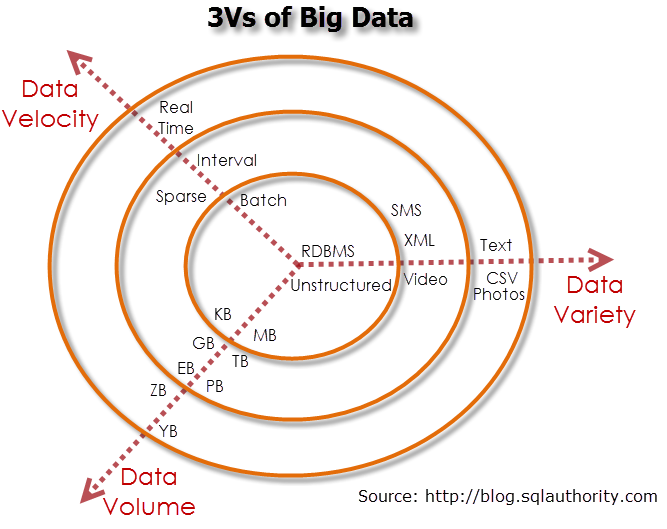
\includegraphics[width=0.8\linewidth]{images/3vs}\caption{3vs data model}\label{fig:3vs}\end{center}\end{figure}
\parindent 0pt
The characteristics of each property illustrated in figure \ref{fig:3vs} are defined as: \textbf{Volume} - The vast amounts of data generated every second. With the creation and storage of large quantities of data, the scale of this data becomes progressively vast. \textbf{Velocity} -  The speed at which new data is generated and the speed at which data moves around emphasising the ``timeliness" of the big data. In order to fully profit from the commercial value of big data, data collection and data examination must be conducted promptly . \textbf{Variety} - This characteristic alludes to the various types of data we can now use; semi-structured and unstructured. Examples being ``audio, video, webpage and text as well as traditional structured data" \cite{bigdata}.

\parindent 15pt
Big data is a term becoming increasingly common in business and society. Overcoming obstacles and implementing effective, actionable Big Data strategies is key for successful big data management. In recent years, a fourth category was introduced: \textbf{Veracity} - Data inconsistencies and incompleteness result in data uncertainty and unreliability. Subsequently this creates a new challenge, keeping data organised \cite{bigdata}.

The final and considered by many to be the most important \textit{V} of big data, is \textbf{Value}. ``All the volumes of fast-moving data of different variety and veracity have to be turned into value" \cite{ibm}. One of the biggest challenges faced by organisations, is having the ability to turn data into something useful. It can be an easy trap to fall into; a business aiming to embark on big data initiatives, without a clear understanding of cost and benefits \cite{bigdata}. Thus, the importance of establishing clear and achievable business objectives.

\begin{figure}[h]\begin{center}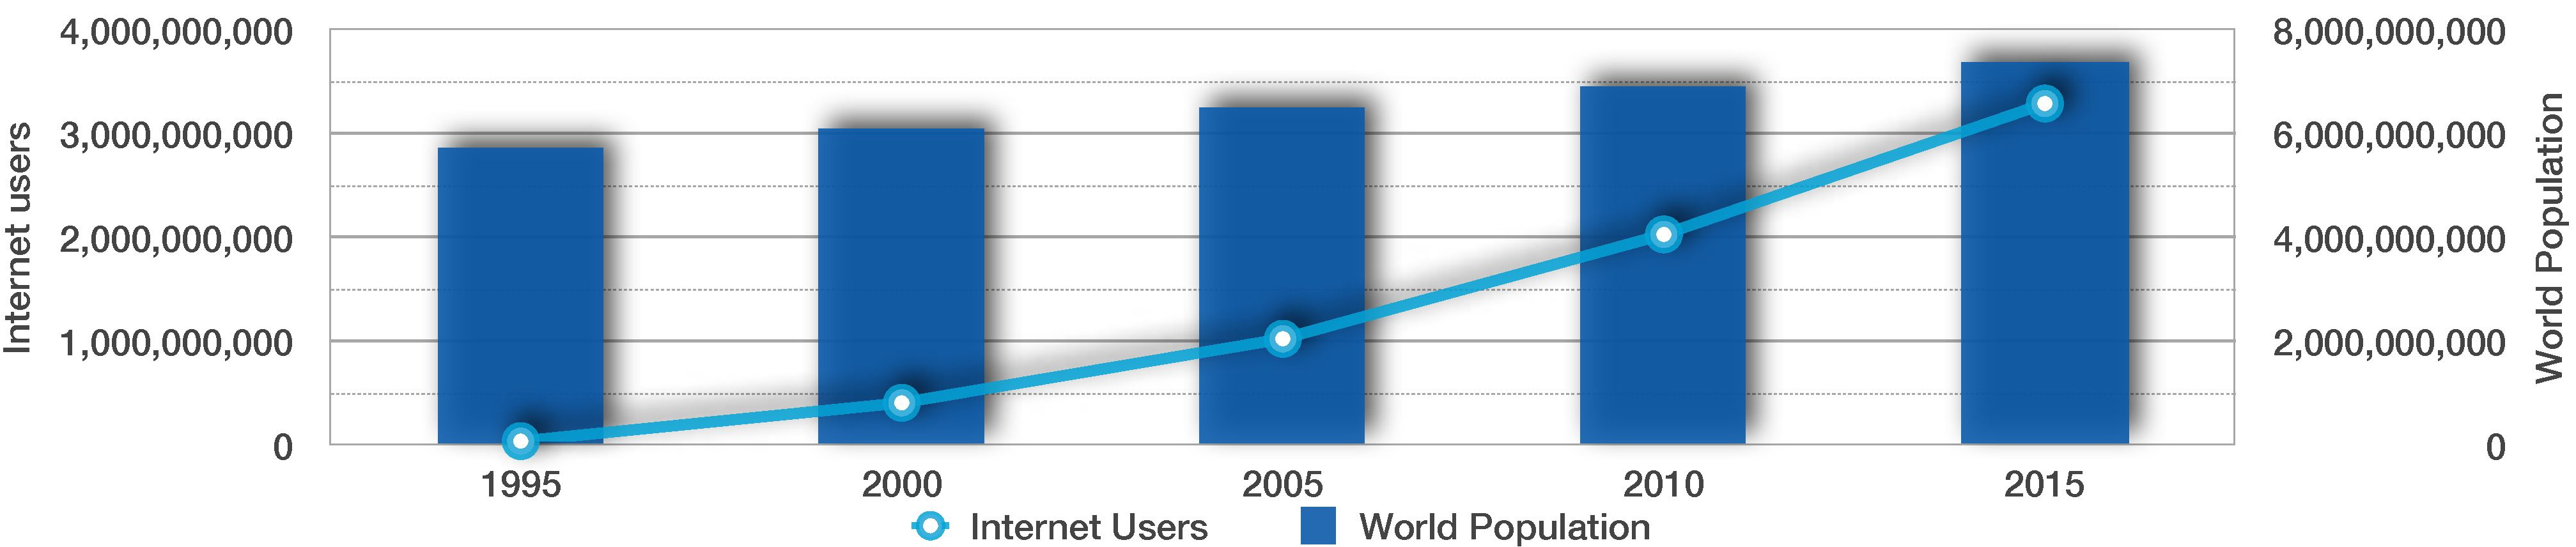
\includegraphics[height=5cm,width=1\linewidth]{images/worldpopgraph}\caption{World population vs Internet users}\label{fig:worldpop}\end{center}\end{figure}
The amount of data produced has dramatically increased from when Laney first introduced the 3vs model in 2001. This is in no small part due to the availability and accessibility of the internet. In 1995 the internet had on average 45 million users, 1\% of the worlds population. This figure increased to over 1 billion people with internet access worldwide in 2005, and by 2010 nearly 2 billion; 30\% of the worlds population. The latest figures show, that in 2015 the penetration of the internet reached 3 billion people; 40\% of the entire population. Social media sites such as Facebook, Twitter, Snapchat, Instagram and Pinterest are some of the main contributors in generating large volumes of user data. Facebook boast a staggering 1 million links shared, 2 million friend requests and 3 million messages sent on average every twenty minutes \cite{statref}. The graph in figure \ref{fig:worldpop} illustrate the continual growth of internet accessibility as a whole.

\section{Extract Transform Load}\label{etlprocess}
A requirement of this project is to extract, manipulate and process multiple datasets. This process is commonly known as Extract Transform Load (ETL). A basic definition of the ETL process is: pulling data from one database, refactoring the composition of the data and loading it into another database. While the name ETL implies there are 3 main stages - extract, transform and load - the procedure in its entirety is a much broader and expansive process. Despite this, the procedure is split into these three stages. Figure \ref{fig:etl} illustrates the ETL process. Data comes from a source, for example a file or database management system. It is then transformed into the required format for a successful load. \begin{figure}[h]\begin{center}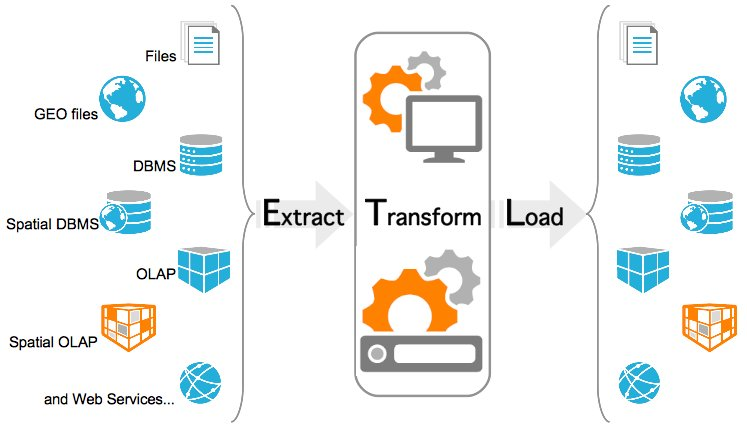
\includegraphics[width=0.8\linewidth]{images/etl.jpg}\caption{ETL process}\label{fig:etl}\end{center}\end{figure}

\subsection{Extract}
Extract is the first step in the ETL procedure. Data is read from a source system and makes it available for processing. The main objective of the extract stage, is to retrieve all the required data from a source system using as little resources as possible \cite{etlref1}. It is common when data is extracted from a source system it will be in a different structure and format to that of the target system. The extract stage provides an opportunity to cleanse the data from the source system, as often there will be redundant or irrelevant data in the dataset which is not required.

\subsection{Transform}
Transform is where the extracted data is manipulated from its previous state and converted into a target system format. This step involves the application of a set of rules or functions to transform the data from source to target. As well as the applied rules and functions, during the transformation stage it is responsible for the validation of records. This is provides one with the opportunity to remove unnaceptable records. ``The most common processes used for transformation are conversion, clearing the duplicates, standardizing, filtering, sorting, translating and looking up or verifying if the data sources are inconsistent" \cite{etlref2}.

\subsection{Load}
Load completes the three step procedure and is where data is written into the target system. There are multiple ways in which data is loaded into a system using the ETL methodology. One of which is to physically insert the data. For example, if the target repository is a SQL database, one can insert the data as a new row using the relevant ``INSERT'' statement. An alternative manually loading the data is to use an ETL tool which has the capability to ``...link the extraction, transformation, and loading processes for each record from the source" \cite{etlref2}. Depending on the technique applied, the load step of the process can become the most time consuming.

\section{NoSQL}\label{nosql}
NoSQL is labeled as a next generation database, known to most as ``Not only SQL'' \cite{nosql1}. However, this definition insinuates its defiance against the industry standard, SQL. NoSQL was originally developed in 1998 by Carlo Strozzi; a member of the Italian Linux society. Strozzi's initial intention was to create a non-relational, widely distributable and highly scalable database system. Strozzi named the systems NoSQL to merely state it does not express queries in the traditional SQL format.

Sadalage and Fowler believe the definition we commonly refer to as NoSQL, comes from a 2009 conference in San Fransisco, held by software developer Johan Oskarsson. Sadalage and Fowler recall Oskarssons desire to generate publicity surrounding the event, and in an attempt to do so, devised the twitter hashtag ``NoSQL Meetup''. The main attendees at the conference debrief session were Cassandra, CouchDB, HBase and MongoDB, and so the association stuck \cite{nosql1}.

NoSQL solutions are not bound by a definitive schema structure thus they are schema-less. This permits the ability to freely adapt database structures and records without considering model changes. This is extremely effective when dealing with varying data types and data sets. In comparison to the traditional relational database model, tackling this issue often resulted in ambiguous field names  \cite{nosql1}.

\subsection{Distributed Systems and Data Transactions}\label{distrosystems}
\subsubsection{Brewer's CAP Theorem}\label{cap}
In the late 1990s, computer scientist Eric Brewer formulated what is known-as CAP theorem \cite{toad}. CAP theorem suggests, that it is impossible for distributed computer systems to provide all of the following three guarantees at the same time:
\begin{itemize}
\item \textbf{Consistency}: All nodes have a consistent view of the system \cite{toad}.
\item \textbf{Availability}: A guarantee that every read/write is acted upon \cite{toad}.
\item \textbf{Partition-tolerance}: The system will always operate despite arbitrary partitioning as a result of network failures \cite{toad}.
\end{itemize}
The proof of Brewer's theorem states that one can only achieve two out of the three guarantees, and this decision comes at a trade-off. The proof of Brewer's theorem goes as follows:
\begin{itemize}[leftmargin=*]
\item For the sake of argument, there are two nodes, one named N1 and the second named N2. They both contain the same dataset (data replication) and are on either side of a partition:
\end{itemize}
\begin{itemize}
\item[--] To ensure both nodes have the same up-to-date view neither node can allow any changes or updates. Thus lose Availability.
\item[--] If there is a change on node 1 then in this scenario node 2 can not view this change, therefore Consistency is lost.
\item[--] Thus only when the two nodes can communicate can Availability and Consistency be guaranteed. However, this will come at a cost of Partition-tolerance.
\end{itemize}
Figure \ref{fig:venncap} below is a Venn diagram illustrating the relationship between the three principles.
\begin{figure}[h]\begin{center}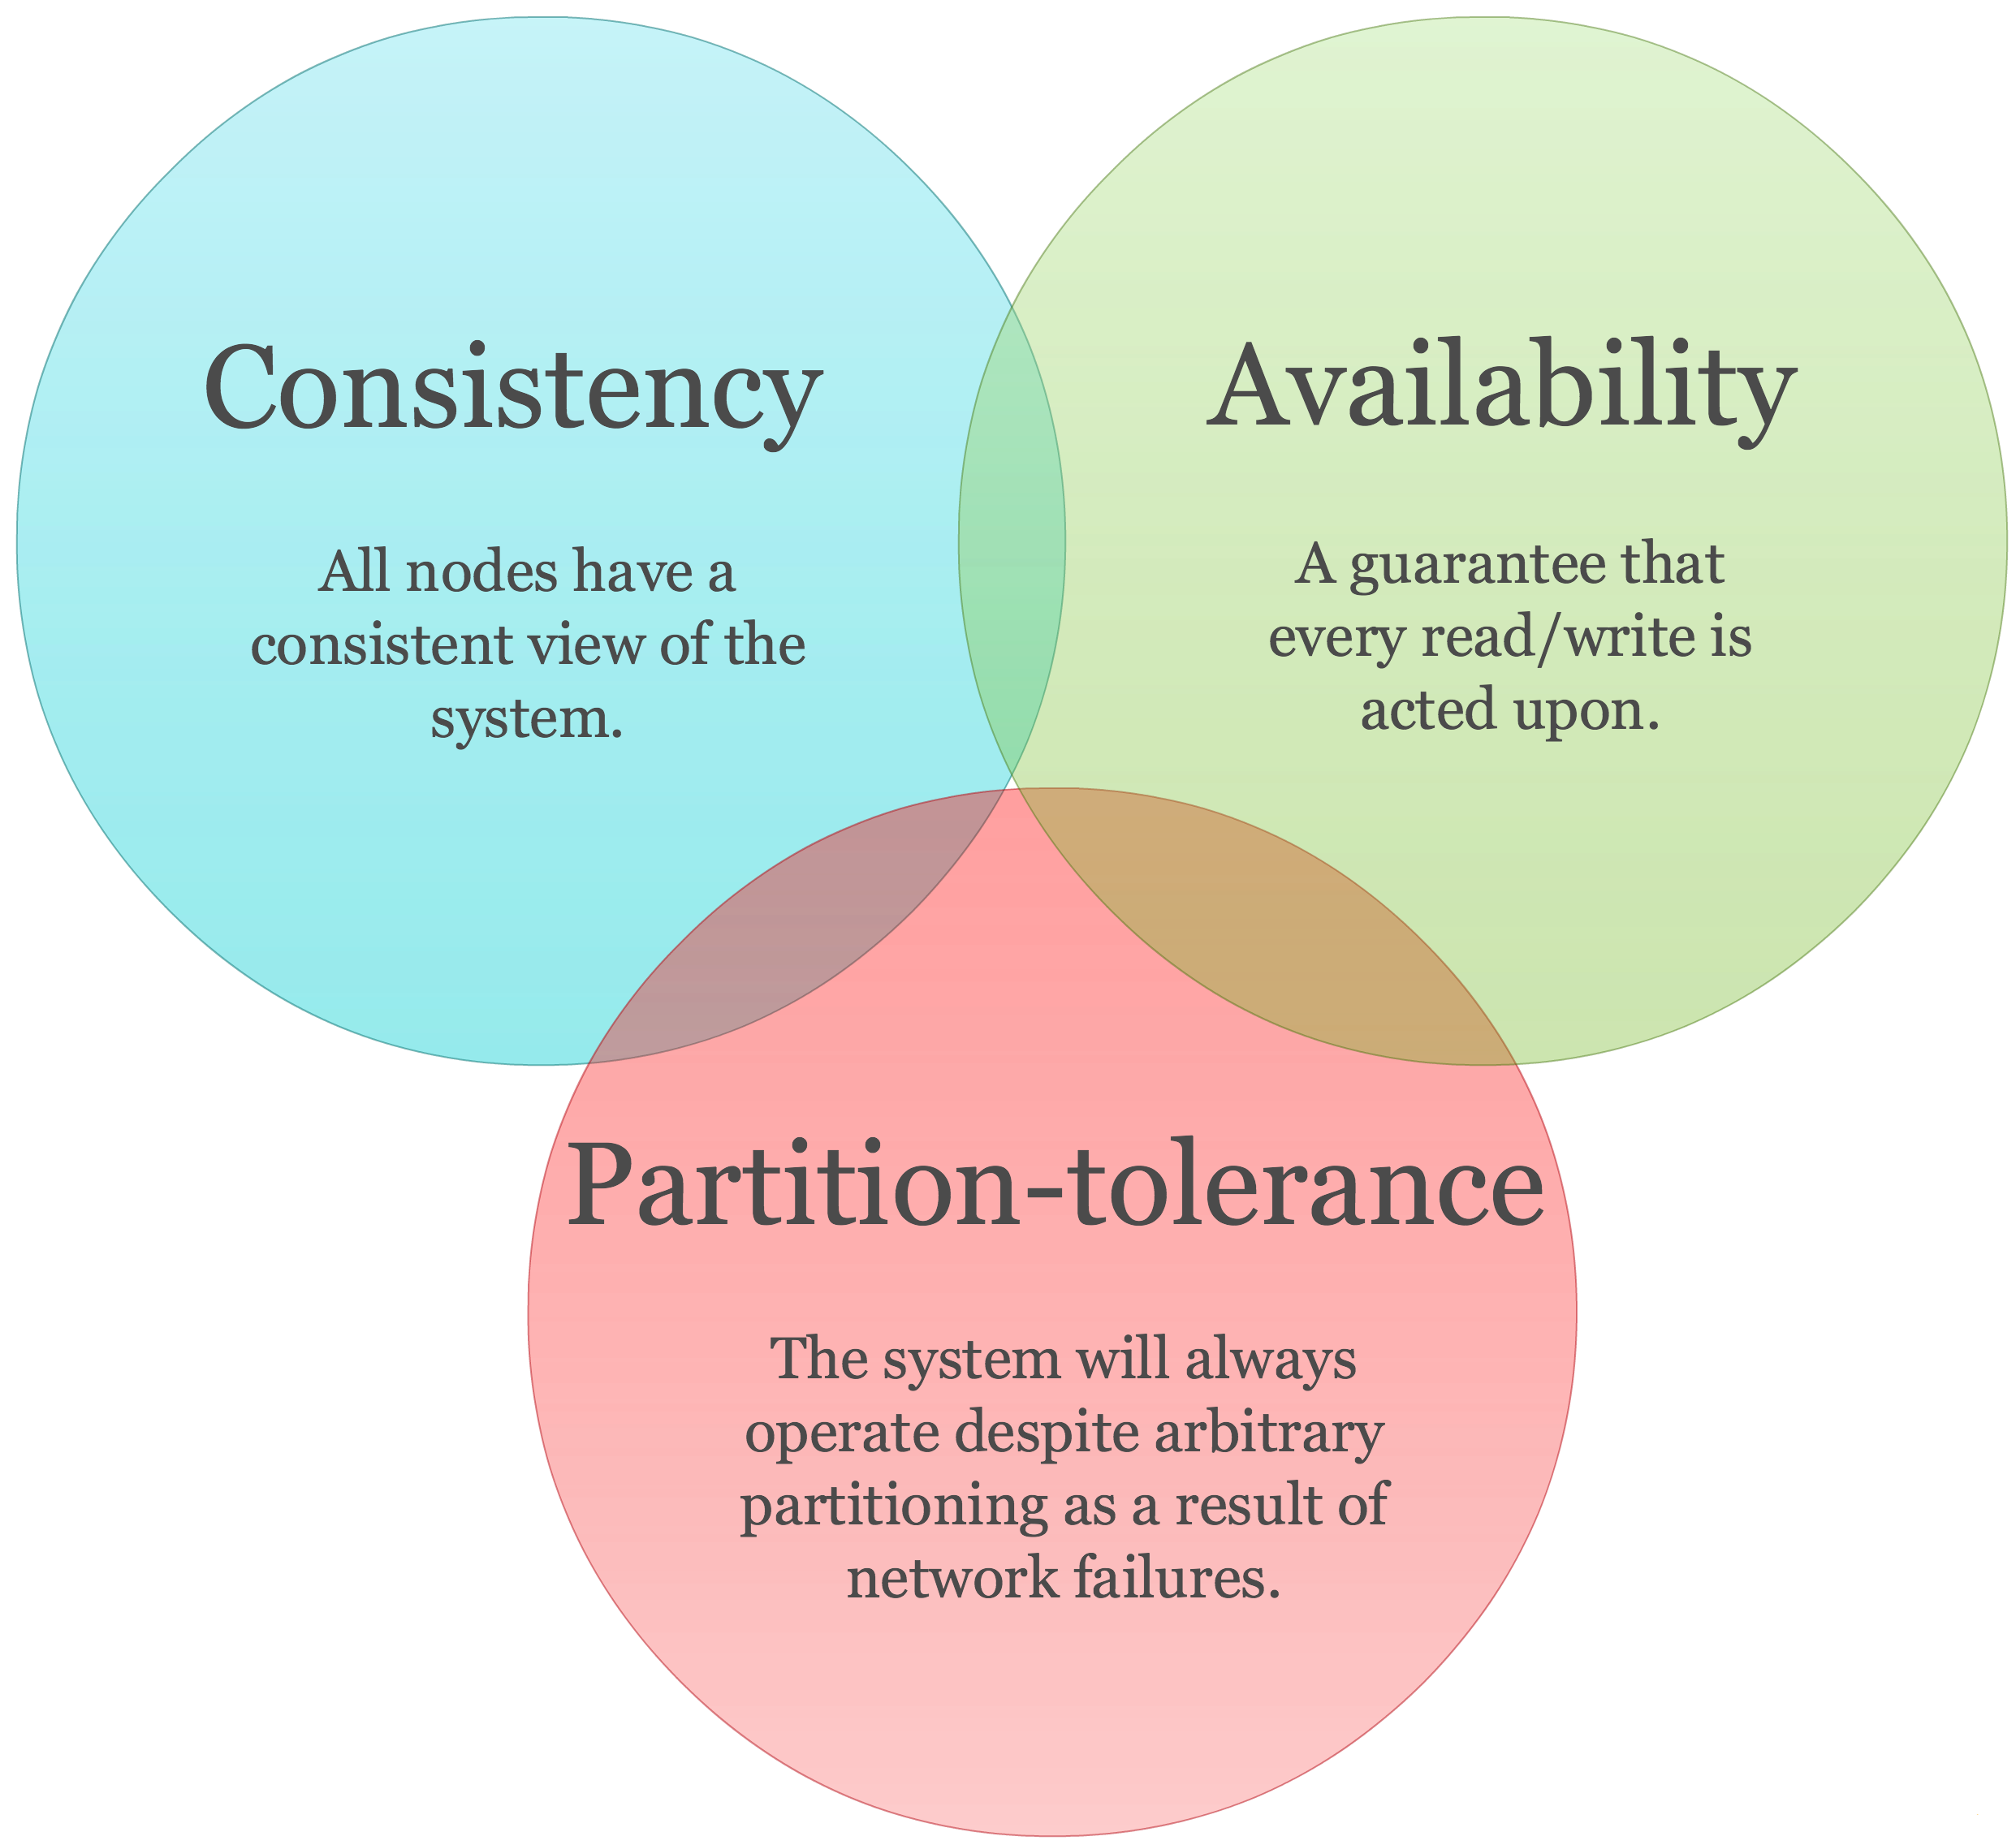
\includegraphics[width=1\linewidth]{images/venncap}\caption{Venn diagram of Brewer's CAP Theorem}\label{fig:venncap}\end{center}\end{figure}

\subsubsection{ACID Transactions}\label{acid}
When discussing database management systems, a transaction is a term which refers to a single logical operation performed on data. For example, transferring money from one bank account to another. The term ACID, coined in the 1983 by Andreas Reuter and Theo Härder, describes the properties of a reliable transaction system \cite{acid}. The acronym ACID can be defined as follows:

\begin{itemize}
\item \textbf{Atomicity}: Transactions are ``all or nothing''. If one part of the transaction fails, then the entire transaction fails cleanly.
\item \textbf{Consistency}: Data written to the database complies with rules and ensures constraints are not broken. Any transaction will bring the database from one valid state to another \cite{acidtrans}.
\item \textbf{Isolation}: Ensures parallel transactions act as if sequential (one after the other).
\item \textbf{Durability}: The system will remember a change once a transaction has been committed.
\end{itemize}

Transactional operations are used for guaranteeing these properties by grouping related actions together. A group of operations can be atomic, deliver consistent data, be isolated from other operations, and be durably recorded \cite{acidtrans}.

\subsubsection{Distributed Database}\label{distributeddb}
A distributed database comprises of two or more data files located at different sites or servers on a computer network \cite{dd}. An advantage of using a distributed database, is that multiple users can access a portion of the database at different locations, locally and remotely without obstructing one another's work. It is pivotal for the distributed database system to periodically synchronise the scattered databases, to ensure that they all have consistent data \cite{dd}. For example, if a user updates or deletes data, it is essential this change is mirrored on all databases. This ability to remotely access a database from all across the world, lends itself to not only multinational companies, but also start-up businesses which recruit the expertise of others from various locations.

\subsection{Database Classification}\label{dbclass}
One of the first decisions to be made when selecting a database, is the characteristics of the data one is intending on storing \cite{nosql2}. There are a multitude of options available with many different classifications. The following sections discuss a subset of these which are relevant to the project.

\subsubsection{Document-Oriented Database}
Document-orientated databases(DODB) are designed for storing, retrieving and managing document files such as XML, JSON and BSON (binary JSON). The documents stored in a DODB model are data objects, which describe the data in the document, as well as the data itself. \begin{figure}[H]\begin{center}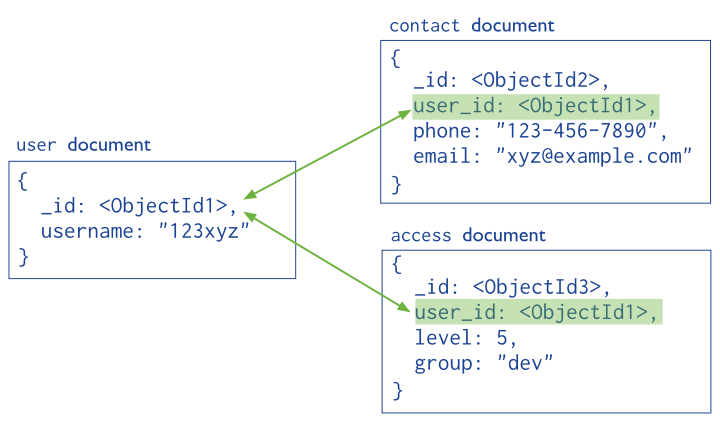
\includegraphics[width=0.75\linewidth]{images/mongodbmodel}\caption{MongoDB document}\label{fig:mongo}\end{center}\end{figure} Figure \ref{fig:mongo} illustrates an example document stored in the most popular DODB, MongoDB. The data is a recognisable JSON format, and the relationships in the document are between common variable values.

\subsubsection{Graph-Orientated Database}
A graph database is a form of NoSQL database solution, that uses graph theory to store, map and query relationships. A graph is a collection of nodes connected by relationships. ``Graphs represent entities as nodes and the ways in which those entities relate to the world as relationships" \cite{gd}. The formation of the graph database structure is extremely useful and eloquent. It permits clear modelling of a vast and often ecliptic array of data types \cite{gd}. An example of data represented in a graph structure, is the Twitter relationship model. 

Figure \ref{fig:twitter} illustrates the nodes involved in a standard tweet and the relationship link between them. The labelled nodes indicate the various operations which are involved in a single tweet. One interpretation of figure \ref{fig:twitter}, is that a user posts a tweet using the Twitter application (App), mentions another user, includes a hash-tag and a link.

\begin{figure}[H]\begin{center}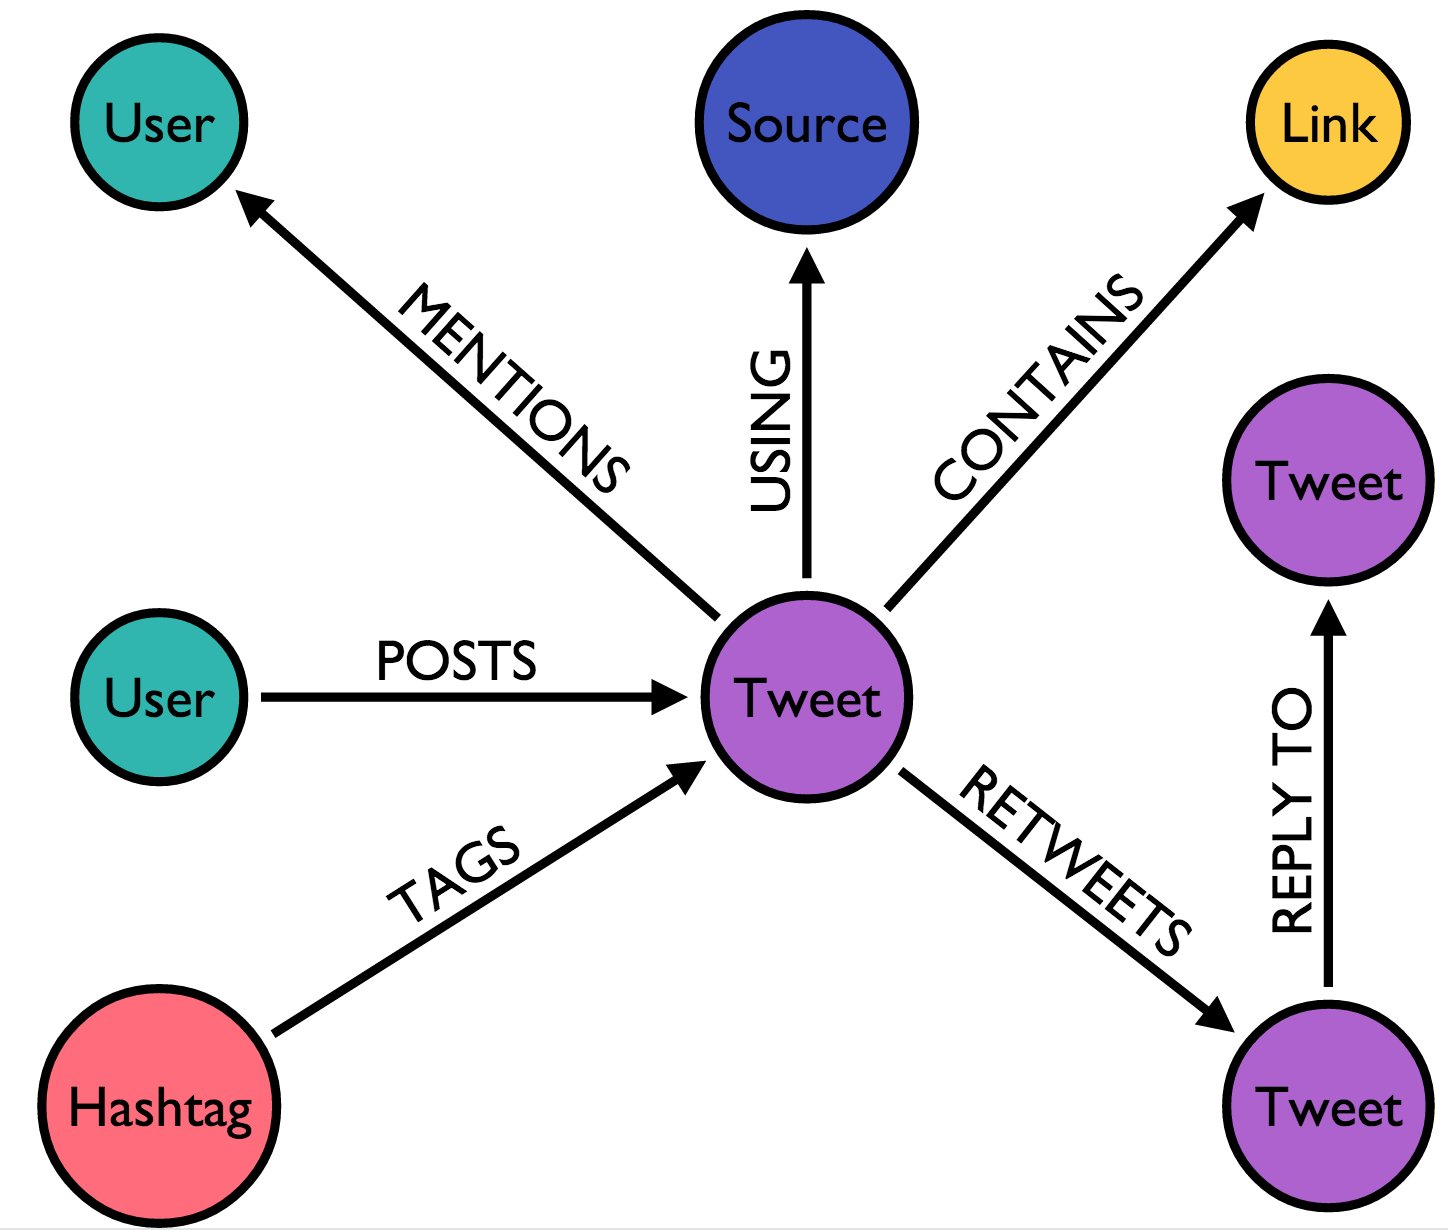
\includegraphics[width=0.5\linewidth]{images/graphdb_twitter}\caption{Example tweet data relationship}\label{fig:twitter}\end{center}\end{figure}

\subsubsection{Column-Orientated Database}
A column-orientated database (CODB) is a database management system which stores data tables as columns, rather than rows. The main objective of a CODB, is to write and read data from the hard disk efficiently in an attempt to speed up querying time. A CODB has the ability to self index. This uses less disk space than RDBMS which holds the same data. A CODB can also be highly compressed, resulting in aggregate functions such as MIN, MAX and SUM to be performed extremely quickly \cite{cd}.

\begin{figure}[H]\begin{center}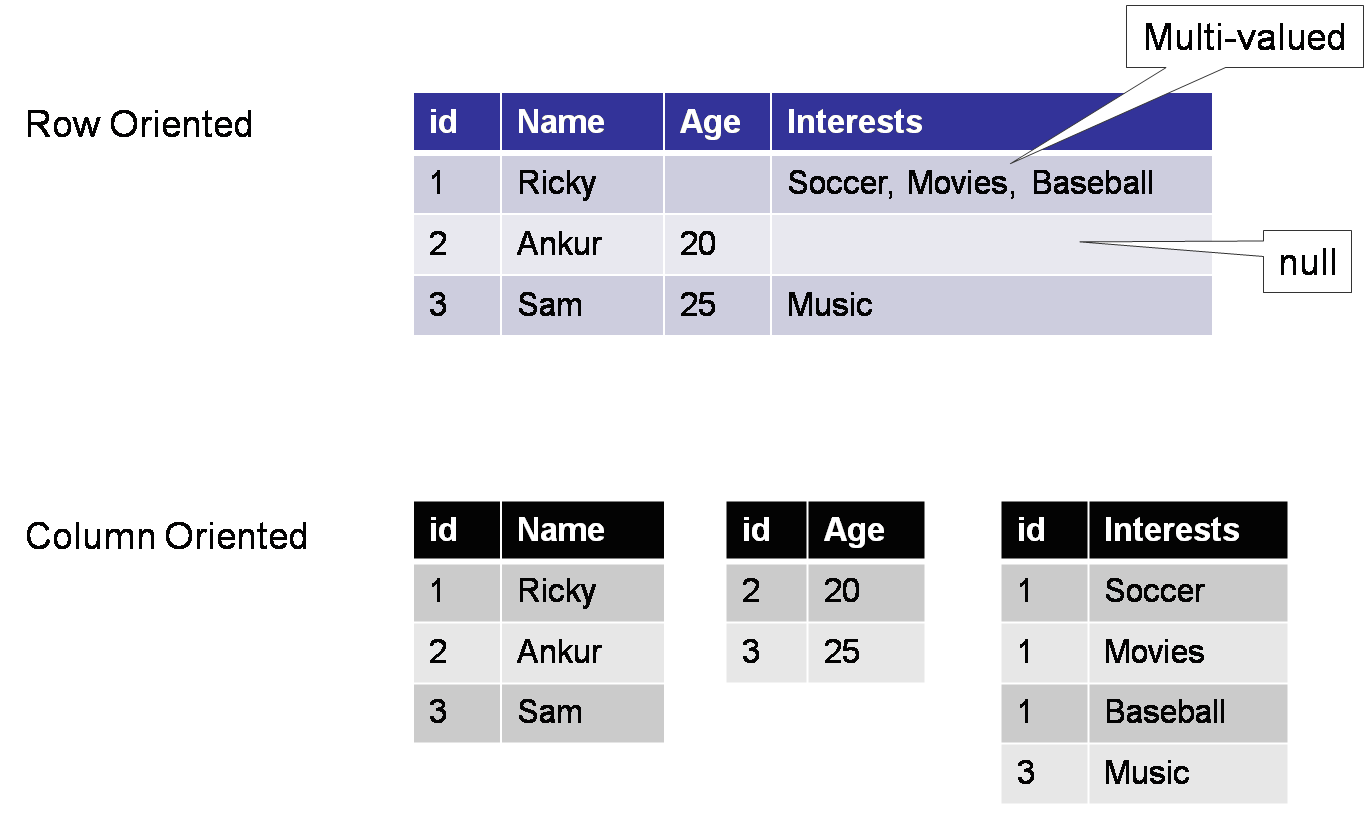
\includegraphics[height=7cm,width=0.75\linewidth]{images/codb}\caption{Column orientated database example}\label{fig:cod}\end{center}\end{figure}

Figure \ref{fig:cod} illustrates the comparison of a relation data model against a CODB model. Within the row based model, the data contains both multiple values per record and NULL values. However, in the CODB model, NULL values are not required as each record contains a minimum and maximum of one value.

\section{Relational Database}
A relational database is a collection of data items organised as a set of tables, records and columns from which data can be accessed or reassembled in many different ways \cite{rdb}. The connected tables are known as relations and contain one or more columns which comprise of data records called rows. Relations can also be instantiated between the data rows to form functional dependencies.

\begin{itemize}
\item One to One: One table record relates to another record in another table.
\item One to Many: One table record relates to many records in another table.
\item Many to One: More than one table record relates to another table record.
\item Many to Many: More than one table record relates to more than one record in another table.
\end{itemize}


\section{Technology Evaluation}\label{techeval}
\subsection{MySQL}\label{mysql}
MySQL is a freely available, open source relational database that uses the Structured Query Language (SQL) programming language. SQL queries are used to perform tasks such as update or retrieve data in a database. The queries are in the form of command line language which include keyword statements such as SELECT, INSERT and UPDATE. MySQL is commonly used for Web applications; its speed and reliability being a key feature. The MySQL database stores data in tables; a collection of logically related, structured data. MySQL allows multiple users to manage and create numerous databases.

MySQL adheres closely to the ACID model. This is to ensure results are not distorted by uncontrollable events such as software crashes and hardware malfunctions. A MySQL component used to interact with the ACID model is the InnoDB storage engine. To provide \textbf{Atomicity}, InnoDB uses transactions, \textbf{Consistency} InnoDB uses internal processing to protect data crashes, \textbf{Isolation} again involves transactions and finally \textbf{Durability} involves MySQL software interacting with ones hardware configuration \cite{mysqlacid}.

\subsection{MongoDB}\label{mongo}
MongoDB is an open source, cross-platform, document-orientated database (DODB). The premise for using MongoDB is simplicity, speed, flexibility and scalability \cite{md}. Its ever growing popularity, specifically amongst programmers, stems from the unrestrictive and flexible DODB model which gives one the ability to query on all fields. MongoDB also boasts instinctive mapping of objects in modern programming languages \cite{md}. MongoDB stores documents in a file format named BSON; a binary extension of JSON. MongoDB uses a query language called CRUD (Create, Read, Update and Delete). CRUD uses the field and value parameters of the JSON document to match clauses in a given query. The output of a query is given in a JSON format.

A record in MongoDB is known as a document; a data structure composed of field and value pairs. Each document is stored in a Collection; a grouping of documents. The values of fields can include other documents, arrays and arrays of other documents. This is known as an embedded document. In order to avoid de-normalisation and data duplication, one can embed a document within a document. This allows one to capture relationships between values by storing it in logically similar documents. The alternative to this, is to have multiple collections of documents and join them using a common ``\_id'' value. However, this method has an effect on the implementation and querying of the data model; discussed in detail in section \ref{mongodesign}.

The key features of using MongoDB are its high performance data persistence, high availability and automatic scaling \cite{md}. As a result in terms of the CAP data model, MongoDB sits firmly in the Consistency and Partition-tolerance (CP) section of the Venn diagram. However, this is tune-able to be Consistency and Availability (CA) by configuring the system to read from the secondary.

\subsection{Neo4j}\label{neo}
Neo4j is an open-source, NoSQL GDB which imposes the Property Graph Model. The team behind the development of Neo4j describe it as an ``An intuitive approach to data problems" \cite{ndweb}. One of the reasons why Neo4j is favoured predominantly amongst database administrators and developers, is its efficiency and high scalability. This is in part due to its compact storage and memory caching for graphs. ``Neo4j scales up and out, supporting tens of billions of nodes and relationships, and hundreds of thousands of ACID transactions per second" \cite{ndweb}. This is an interesting aspect of Neo4j, as most NoSQL solutions are tailored towards the Consistency and Partition-tolerance systems. However, while Neo4j has been designed with ACID transactions in mind, in terms of the CAP theorem, it would guarantee Consistency and Availability (CA). This is categorisation which most relational database management systems fall into.

The Neo4j query language Cypher, is based on SQL. It shares much of the same syntax which has similar semantic value. The key features of Neo4j which lends itself to users, developers and database administrators are its ability to establish relationships on creating, the equality of relationships permits the addition of new relationships being created after initial implementation at no performance cost and its use of memory caching for graphs which allows efficient scaling.

\subsection{Apache Cassandra}\label{cassandra}
Apache Cassandra is an open source, column-orientated DDB, that is designed for storing and managing vast amounts of data across multiple servers. ``Apache Cassandra is a highly scalable, high-performance distributed database designed to handle large amounts of data across many commodity servers, providing high availability with no single point of failure" \cite{cassandra}. \begin{figure}[H]\begin{center}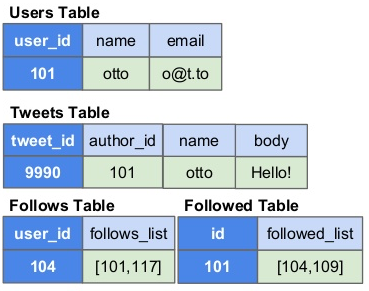
\includegraphics[height=6.5cm,width=0.6\linewidth]{images/cassandramodel}\caption{Example Cassandra record}\label{fig:cass}\end{center}\end{figure}Cassandra uses a query langauge called Cassandra Query Language (CQL). As with Neo4j, CQL based on SQL semantics with some additional features. Apache Cassandra define the key features of their database management system as ``continuous availability, linear scale performance, operational simplicity and easy data distribution across multiple data centres and cloud availability zones" \cite{cassandra}. In terms of the CAP theorem, it is as a result of its strong consistency, which guarantees Cassandra, Consistency and Partition-tolerance by default. Figure \ref{fig:cass} illustrates an example record stored in a Cassandra database.

\section{Data Source and Representation}\label{datasource}
The datasets used to populate the databases are called EMAP and EMAGE. They are freely available, anatomical ontologies of the developmental stages of a mouse embryo. The datasets were chosen for this project as my supervisors have much experience in the field and were able to assist me with any queries I had regarding the data. The size and granularity of the EMAP and EMAGE datasets meet the required criteria to test the database solutions. They will also facilitate the need to explore the limitations of each database and pose insight into the overall performance of each system.

\subsection{EMAP}
The Edinburgh Mouse Atlas Project (EMAP) is an ongoing research project to develop a digital atlas of mouse development. The objective of the EMAP, is to implement a digital model of mouse embryos for each time stage in development \cite{emap}. The collated model embryo data is then used to form a database, from which further research can be conducted and experiments can be mapped.
 
Each time step in the digital model are named Theiler Stages, inspired by the research conducted by Karl Theiler. A Theiler Stage defines the development of a mouse embryo by the form and structure of organisms and their specific anatomical structural features. There are 26 individual Theiler Stages which define the growth and evolution of the mouse embryo. A Theiler Stage comprises of both the anatomical developmental stage definition and the estimated length of time since conception. Each Theiler Stage also provides a brief description of the anatomy, and any significant changes between the current and previous stage.

Theiler proposed using this scheme, as embryos at the same developmental age can have evolved at different rates. Therefore, they can potentially exhibit different structural characteristics. The EMAP has developed a collection of three dimensional computer models which illustrate and summarise each Theiler Stage \cite{emap}.

The anatomy at each Theiler Stage has an associated ontological representation. Each representation provides an alternative aspect of the evolution of a mouse embryo which corresponds with a respective Theiler Stage. A Theiler Stage is just one method used to define the age of the developing embryo. The term DPC or Days Post Conception, uses the literal number of days since the embryo was created to define its developmental stage. For example, ``12.5 dpc'' means there has been 12 and a half days since conception.

The abbreviated term EMAP carries a certain amount of ambiguity as it is refers to the name of the project, and the name of the original anatomy ontology. For the purpose of this project one the main anatomies to be used is the aggregated, non-stage specific, Edinburgh Mouse Atlas Project Abstract (EMAPA) anatomy.

There are a number of terms used in the EMAP datasets which may be unfamiliar to those who do not have an understanding of the biological field. One basic term is a ``gene''; a hereditary unit consisting of a sequence of DNA \cite{emap}. ``Gene expression'' is the specific activity of a gene, when a segment of DNA is copied into RNA. Another term is an ``assay''. A single experiment can comprise of one or more assays. For example, if a biologist is researching a specific gene in a finger, this can be split into multiple sections. A ``probe'' is used to detect DNA and RNA on membranes and is also used when preparing for ``in situ'' experiments. ``In situ'' is a Latin term for `in place'. With regard to this dataset it refers to the original position of the anatomy when being experimented on \cite{emap}. For example, if researching a finger, instead of taking it off the hand and crushing it down to find the genes inside, it remains in-tact with the hand.

\subsection{EMAP anatomy}
The EMAP ontology was originally developed to deliver a stage-specific anatomical structure, for the developing laboratory mouse. As the EMAP research has progressed, the ontology has followed suit and is continually under development.

The original EMAP ontology consists of a series of relational components organised in a hierarchical tree structure which utilise ``part-of" relations and subdivisions which encompass each Theiler Stage \cite{emap}. The intention behind the implementation of the original ontology structure, was to ``...describe the whole embryo as a tree of anatomical structures successively divided into non-overlapping named parts" \cite{emap}.

Each Theiler Stage component has an appropriately named term label, known as the \textit{short name}. These labels describes each respective component. Each Theiler Stage also has a \textit{full name}, which comes in the form of the components entire hierarchical path \cite{emap}. Neither the \textit{full} nor \textit{short} anatomical name of each component are required to be distinct and can appear in several Theiler Stages. Therefore to avoid ambiguity, each component can be addressed by a unique identifier. The unique identifier is in the form of the anatomy, followed by a number (EMAP:number). For example, ``choroid plexus" is the short name of TS20/mouse/body region/head/brain/choroid plexus and has a has unique identifier of EMAP:4218.

\begin{figure}[H]\begin{center}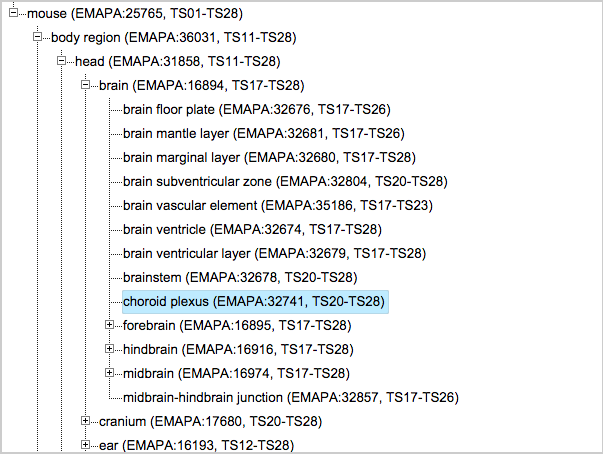
\includegraphics[width=1\linewidth]{images/emapachoroidplexus}\caption{EMAPA data structure}\label{fig:emapa}\end{center}\end{figure}

The EMAP hierarchical structure facilitates the need for basic data annotation and integration. However, a combination of the lack of hierarchical views, missing or poorly represented Theiler Stages, and label name ambiguity, exposed the limitations of the EMAP structure. As a result, the need for a hybrid ``abstract" version of the anatomy was identified and subsequently developed; EMAPA \cite{emap}. Thus the EMAPA anatomy will be the used as a data source for this work.

The research surrounding the EMAP resource is continually being developed, thus the growth of the project as a whole is progressively increasing with the richness of data at the heart \cite{emap}.

\subsection{EMAPA dataset}\label{emapaanatomy}
EMAPA is a refined and algorithmically developed non-stage specific anatomical ontology abstract representation of the EMAP anatomy. The EMAPA implementation replaces the EMAP hierarchical tree structure for a directed acyclic graph structure - a graph in which it is impossible to start at some vertex v and follow a sequence of edges that eventually loops back to v again. Thus enabling the ability to represent multiple parental relationships and other forms of ``is-a" relations \cite{emap}.

Each anatomical component in the EMAPA anatomy is identified as a single term. These terms are coupled with the start and end Theiler Stage at which the component is considered to be present in the developing embryo \cite{emap}. To enhance user experience, the EMAPA anatomy  adopts an alternative naming convention from the EMAP anatomy, replacing full path names for components, to \textit{``print names"}. Using the above example for comparison, ``EMAP:4218" in the EMAP anatomy becomes ``TS20 brain choroid plexus" in EMAPA. This naming convention supplements the requirement of uniqueness and is easy to understand.

\subsection{EMAGE dataset}
EMAGE is a database consisting primarily of image data of \textit{in situ} gene expression data of the developing mouse embryo. The EMAGE description includes a text-based component but the unique aspect of EMAGE is its spatial annotation focus \cite{emap}. The data is sourced from in the community. It is is then taken by curators, who monitor the EMAGE project. The curators then design a standardised way that allows data query and exchange. ``Sites of gene/enhancer expression in EMAGE are described by denoting appropriate regions in the EMAP virtual embryos where expression is detected (and not detected) and also describing this information with an accompanying text-based description, which is achieved by referring to appropriate terms in the anatomy ontology" \cite{emap}.